\documentclass[twocolumn,prd,aps,superscriptaddress,preprintnumbers,tightenlines,showpacs,nofootinbib,eqsecnum,amsfonts,amsmath,longbibliography]{revtex4-1}
\usepackage{epsfig}
\usepackage{graphics}
\usepackage{graphicx}
\usepackage[dvipsnames]{xcolor}
\usepackage{bm}
\usepackage{txfonts}
% \usepackage{newtxtext}
% \usepackage{newtxmath}
\usepackage{natbib}
% \usepackage{amssymb}
\usepackage{xspace}
\usepackage[normalem]{ulem} % To get strikethrough (\sout)
\usepackage[colorlinks]{hyperref}
\usepackage[caption=false]{subfig}
\usepackage{booktabs}
\usepackage{url}
\usepackage{float}
\usepackage[bottom]{footmisc}
\usepackage{lineno}
\usepackage{mathrsfs}
\usepackage{makecell}
\usepackage{microtype}

\usepackage{tikz}

% -----------
% Bibligraphy
% -----------
\AtBeginDocument{%
    \newwrite\bibnotes
    \def\bibnotesext{Notes.bib}
    \immediate\openout\bibnotes=\jobname\bibnotesext
    \immediate\write\bibnotes{@CONTROL{REVTEX41Control}}
    \immediate\write\bibnotes{@CONTROL{%
    apsrev41Control,author="08",editor="1",pages="1",title="0",year="1"}}
    \if@filesw
    \immediate\write\@auxout{\string\citation{apsrev41Control}}%
    \fi
}


\definecolor{LinkColor}{rgb}{0.75, 0, 0}
\definecolor{CiteColor}{rgb}{0, 0.5, 0.5}
\definecolor{UrlColor}{rgb}{0, 0, 0.75}
\definecolor{rred}{RGB}{218,41,28}
\hypersetup{linkcolor=NavyBlue}
\hypersetup{citecolor=NavyBlue}
\hypersetup{urlcolor=NavyBlue}

\usepackage{perpage}
\MakePerPage{footnote}

\newcommand{\paperone}{Paper~I\xspace}

\newcommand{\h}{\mathpzc{h}}
\newcommand{\Hhat}{\hat{\mathpzc{H}}}
\newcommand{\B}{\mathpzc{B}}
\newcommand{\hlm}{\mathpzc{h}_{\ell m}}
\newcommand{\xilm}{\xi_{\ell m}}
\newcommand{\Ylm}{{Y}^{-2}_{\ell m}}
\newcommand{\Y}{{Y}^{-2}}
\newcommand{\hc}{h_\times}
\newcommand{\hp}{h_+}
\newcommand{\Fc}{F_\times}
\newcommand{\Fp}{F_+}
\newcommand{\Mf}{M_f}
\newcommand{\cA}{\mathpzc{A}}
\newcommand{\lm}{_{\ell m}}
\newcommand{\deff}{d_\mathrm{eff}}
\newcommand{\rmi}{\mathrm{i}}
\newcommand{\blambda}{\bm{\lambda}}
\newcommand{\btheta}{\bm{\theta}}
\newcommand{\bxi}{\bm{\xi}}
\newcommand{\bxigr}{\bm{\xi}_{\text{GR}}}
\newcommand{\bxingr}{\bm{\xi}_{\text{nGR}}}
\newcommand{\bzeta}{\bm{\zeta}}
\newcommand{\bs}[1]{\bm{\vec{S}_{#1}}}
\newcommand{\Mo}{M_{\odot}}
\newcommand{\FFe}{\mathrm{FF}_\mathrm{eff}}
\newcommand{\FF}{\mathrm{FF}}
\newcommand{\e}{\mathrm{e}}
\newcommand{\rhoopt}{\rho_\mathrm{opt}}
\newcommand{\rhosubopt}{\rho_\mathrm{subopt}}
\newcommand{\fqnm}{f}
\newcommand{\sigmaqnm}{\sigma}
\newcommand{\n}{\mathbf{n}}
\newcommand*{\skymapscale}{0.5}
\newcommand*{\paramestscale}{0.455}
\newcommand{\df}[1]{\delta f_{\text{#1}}}
\newcommand{\dtau}[1]{\delta \tau_{\text{#1}}}
\newcommand{\fngr}[1]{f_{\text{#1}}}
\newcommand{\taungr}[1]{\tau_{\text{#1}}}
\newcommand{\fgr}[1]{f ^{\text{GR}}_{\text{#1}}}
\newcommand{\taugr}[1]{\tau ^{\text{GR}}_{\text{#1}}}
\newcommand{\pSEOB}{\texttt{pSEOBNR}}
\newcommand{\SEOB}{\texttt{SEOBNR}}

% Modified gravity related
\newcommand{\pd}{\partial}
\newcommand{\dd}{{\rm d}}
\newcommand{\ii}{{\rm i}}
\newcommand{\dV}{{\rm d}^{4}x \, \sqrt{-g} \,}

\newcommand{\lame}{\lambda_{\rm e}}
\newcommand{\lamo}{\lambda_{\rm o}}

% Comment commands
\newcommand{\ag}[1]{{\textcolor{cyan}{{[AG: #1]}} }}
\newcommand{\hs}[1]{{\textcolor{blue}{{[HS: #1]}} }}
\newcommand{\ab}[1]{{\textcolor{green}{{[AB: #1]}} }}

\newcommand{\AEI}{\affiliation{Max Planck Institute for Gravitational Physics (Albert Einstein Institute), Am M\"uhlenberg 1, Potsdam 14476, Germany}}
\newcommand{\UMD}{\affiliation{Department of Physics, University of Maryland, College Park, Maryland 20742, USA}}

\begin{document}

% HS: temporary title. Feel free to add suggestions
% \title{Probing higher-curvature gravity theories from binary black hole ringdown signals}
\title{Black-hole ringdown as a probe of higher-curvature gravity theories}

\author{Hector O. Silva}
\author{Abhirup Ghosh}
\AEI
\author{Alessandra Buonanno}
\AEI
\UMD

\date{\today}


%%%%%%%%%%%%%%%%%%%%%%%
\begin{abstract}
\end{abstract}
%%%%%%%%%%%%%%%%%%%%%%%

\maketitle
% \tableofcontents

%%%%%%%%%%%%%%%%%
\section{Introduction}
\label{sec:intro}
%%%%%%%%%%%%%%%%%

\hs{AB will do this.}

\section{Overview of modified gravity theories}
\label{sec:review_theories}

% We will consider several modified gravity theories as applications of the \pSEOB{}
% waveform model presented in Sec.~\ref{sec:review_pSEOB}.
%
We briefly review which theories we consider, what are the currents
observational constraints in each of them and what we known about the QNMs of
black holes in each of them.

\subsection{scalar-Gauss-Bonnet gravity}
%
This theory is given by the following action,
%
\begin{equation} \label{eq:action_sgb}
    S_{\rm GB} = \frac{1}{16 \pi}
    \int \dV
    \left[
    R - \tfrac{1}{2}(\nabla \varphi)^2
    + \tfrac{1}{4} \ell^{2}_{\rm GB} f(\varphi) \mathscr{G}
    \right],
\end{equation}
%
where $R$ is the Ricci scalar associated with the metric $g_{\alpha\beta}$ and
$\varphi$ is a dynamical scalar field which couples to the Gauss-Bonnet
invariant $\mathscr{G}$,
%
\begin{equation} \label{eq:def_gb}
    \mathscr{G} =
    R^{\mu\nu\rho\sigma}R_{\mu\nu\rho\sigma}
    - 4 R^{\mu\nu}R_{\mu\nu}
    + R^2,
\end{equation}
%
with strength set by the dimensionful coupling constant $\ell_{\rm GB}$ with dimensions
of length.

Different subclasses of this theory are determined by the function $f(\varphi)$
and they can be classified into two classes based on the properties of their black hole solutions.
%
In the first class, the first derivative of the coupling
function $f'(\varphi) = \dd f  / \dd \varphi$ is always nonzero and black holes
are known to always support (secondary) scalar hair.
%
Examples include the shift-symmetric $f \propto \varphi$ and dilatonic
$f \propto \exp(\varphi)$ couplings.
%
In the second class, $f'(\varphi) = 0$ can vanish for some constant $\varphi_0$.
%
In this case, one can show that theory admits the same stationary,
asymptotically flat black hole solution of GR and scalarized black
holes~\cite{Doneva:2017bvd,Silva:2017uqg,Dima:2020yac,Herdeiro:2020wei,Berti:2020kgk}.
%
Examples include the quadratic $f \propto \varphi^2$~\cite{Silva:2017uqg}
and Gaussian $f \propto \exp(-\varphi^2)$~\cite{Doneva:2017bvd} couplings.
%
Here will consider only the dilatonic theory.

Black holes in both classes support monopolar scalar hair and thus, when in binaries,
can source scalar dipole radiation and are therefore prone to be constrained with
GWs observations of compact binaries~\cite{Nair:2019iur,Perkins:2021mhb}.
%
\dots

The calculation of the QNMs in this theory is more complicated than in GR already for
nonrotating black holes. The reason is due to the coupling between scalar field and
the Gauss-Bonnet invariant, which manifests into a coupling between scalar perturbation
and gravitational perturbations of polar parity \dots

\begin{figure}
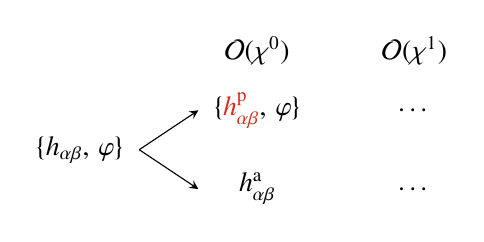
\begin{tikzpicture}[baseline,>=stealth]
    % \draw[help lines, gray] (-4, -2) grid (4, 2);
    \draw[->] (-2.5, 0) -- (-1.75, +0.5);
    \draw[->] (-2.5, 0) -- (-1.75, -0.5);

    \node at (-3.25, 0) {$\{h_{\alpha\beta}, \, \varphi\}$};

    \node at (-1, 1.25) {${\cal O}(\chi^{0})$};
    \node at (-1, +0.5) {$\{ \textcolor{rred}{h^{\rm p}_{\alpha\beta}}, \, \varphi\}$};
    \node at (-1, -0.5) {$h^{\rm a}_{\alpha\beta}$};

    \node at (+1, 1.25) {${\cal O}(\chi^{1})$};
    \node at (+1, +0.5) {\dots};
    \node at (+1, -0.5) {\dots};
\end{tikzpicture}
\caption{Quasinormal modes of black holes in scalar-Gauss-Bonnet gravity.}
\end{figure}

\subsection{dynamical Chern-Simons gravity}

This theory is given by the following action,
%
\begin{equation} \label{eq:action_dcs}
    S_{\rm CS} = \frac{1}{16 \pi}
    \int \dV
    \left[
    R - \tfrac{1}{2}(\nabla \vartheta)^2
    + \tfrac{1}{4} \ell^{2}_{\rm CS} \, \vartheta \, {}^{*}RR
    \right],
\end{equation}
%
where $\vartheta$ is a pseudo-scalar field, which couples
to the Pontryagin density,
%
\begin{equation}
    {}^{*}RR = {}^{*}R^{\mu}{}_{\nu}{}^{\rho\sigma} R^{\nu}_{\mu\rho\sigma},
\end{equation}
%
where ${}^{*}R^{\mu}{}_{\nu}{}^{\rho\sigma}$ is the dual of the Riemann tensor,
defined as
%
${}^{*}R^{\mu}{}_{\nu}{}^{\rho\sigma} =
\tfrac{1}{2} \epsilon^{\mu}{}_{\nu\gamma\delta}
R^{\gamma\delta\rho\sigma}$,
%
and where $\epsilon^{\mu}{}_{\nu\gamma\delta}$ is the Levi-Civita tensor.
%
The coupling between scalar field and the Pontryagin density is set by the
$\ell_{\rm CS}$ with dimensions of length.

The theory admits the Schwarzschild black hole solution of GR, but predicts
that spinning black holes have (secondary) scalar hair, which, unlike in
scalar-Gauss-Bonnet gravity, is dipolar~\cite{Yunes:2009hc,Konno:2009kg}.
%
Consequently, the leading-scalar radiation channel is quadrupolar making this
theory presently unconstrained by from the GWs from the inspiral of black hole
binaries alone~\cite{Nair:2019iur,Perkins:2021mhb}.
%
However, the theory has been constrained by Ref~\cite{Silva:2020acr} through a
combination information of x-ray observations of the isolated neutron star PSR
J0030+0451~\cite{Lommen:2000yt,NANOGrav:2017wvv} by the
NICER~\cite{Riley:2019yda,Miller:2019cac} and gravitational-wave observation of
the binary neutron star event GW170817~\cite{TheLIGOScientific:2017qsa}.

Similarly to the case of scalar-Gauss-Bonnet gravity, the perturbations of nonrotating
black holes in dynamical Chern-Simons gravity also have a coupling between scalar and
metric perturbations. However, the coupling is between the scalar and gravitational perturbations
of axial parity~\cite{Yunes:2007ss,Cardoso:2009pk,Molina:2010fb,Wagle:2021tam}.

\begin{figure}
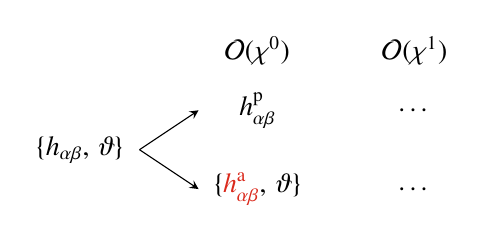
\begin{tikzpicture}[baseline,>=stealth]
    % \draw[help lines, gray] (-4, -2) grid (4, 2);
    \draw[->] (-2.5, 0) -- (-1.75, +0.5);
    \draw[->] (-2.5, 0) -- (-1.75, -0.5);

    \node at (-3.25, 0) {$\{h_{\alpha\beta}, \, \vartheta\}$};

    \node at (-1, 1.25) {${\cal O}(\chi^{0})$};
    \node at (-1, +0.5) {$h^{\rm p}_{\alpha\beta}$};
    \node at (-1, -0.5) {$\{ \textcolor{rred}{h^{\rm a}_{\alpha\beta}}, \, \vartheta\}$};

    \node at (+1, 1.25) {${\cal O}(\chi^{1})$};
    \node at (+1, +0.5) {\dots};
    \node at (+1, -0.5) {\dots};
\end{tikzpicture}
\caption{Quasinormal modes of black holes in dynamical Chern-Simons gravity.}
\end{figure}

\subsection{Effective-field-theory of GR}

This theory is given by the following action,
%
\begin{equation} \label{eq:action_eft}
    S_{\rm EFT} = \frac{1}{16 \pi}
    \int \dd^4x \sqrt{-g}
    \left[ R
    +
    \footnotesize{\sum}_{n \geqslant 2} \ell^{2n - 2} L^{(2n)}
    \right],
\end{equation}
%
where $\ell$ is some length scale, assumed to be small compares to the length
scale associated with a black hole, i.e., $\ell / M \ll 1$, and
$L^{(2n)}$ are corrections to the Einstein-Hilbert term action that
introduce involving higher-order curvature tensors (with $2n$ metric
derivatives).

More specifically, we follow Refs.~\cite{Cano:2020cao,Cano:2021myl} and work up
to dimension-eight operators (i.e., $n=4$),
%
\begin{subequations}
\label{eq:action_mods}
\begin{align}
    L^{(6)} &= \lame R_{\mu\nu}{}^{\rho\sigma} R_{\rho\sigma}{}^{\gamma\delta} R_{\gamma \delta}{}^{\mu\nu}
    \nonumber \\
            &\quad + \lamo R_{\mu\nu}{}^{\rho\sigma} R_{\rho\sigma}{}^{\gamma\delta} \tilde{R}_{\gamma \delta}{}^{\mu\nu},
    \label{eq:s_6}
    \\
    L^{(8)} &= \varepsilon_{1} \mathcal{C}^2
    + \varepsilon_{2} \tilde{\mathcal{C}}^{2}
    + \varepsilon_{3} \mathcal{C} \tilde{\mathcal{C}},
\label{eq:s_8}
\end{align}
\end{subequations}
%
where $\lambda_{\rm o, e}$ and $\varepsilon_{i}$ ($i=1,2,3$) are dimensionless parameters.

Black holes in these theories were found in Refs.~\cite{deRham:2020ejn,Cano:2020cao} for the dimension-six EFT
and in Refs.~\cite{Cardoso:2018ptl} for the dimension-eight EFT.

% where we defined the Gauss-Bonnet and Pontryagin densities, respectively,
% %
% \begin{subequations}
% \begin{align}
%     R^{2}_{\rm GB} &= R_{\mu\nu\rho\sigma}R^{\mu\nu\rho\sigma} - 4 R_{\mu\nu} R^{\mu\nu} + R^2,
%     \\
%     {}^{*}RR &= \tfrac{1}{2} R_{\nu\mu\rho\sigma} {}^{*}R^{\mu\nu\rho\sigma},
% \end{align}
% \end{subequations}
% %
% and where $R_{\mu\nu\rho\sigma}$ is the Riemann tensor
% and $\tilde{R}_{\mu\nu\rho\sigma}$ its dual, defined as
% %
% \begin{equation}
% \tilde{R}_{\mu\nu\alpha\beta} = \tfrac{1}{2} \epsilon_{\mu\nu\rho\sigma} R^{\rho\sigma}{}_{\alpha\beta},
% \end{equation}
% %
% with $\epsilon_{\mu\nu\rho\sigma}$ being the Levi-Civita tensor.

% This action encapsulates various modified gravity theories, which often are studied on their own,
% namely,
% %
% \begin{itemize}
%     \item scalar Gauss-Bonnet gravity (sGB): corresponds to $\alpha_{\rm GB}$
%           nonzero and all other dimensionless coupling constants equal to zero.
%     \item dynamical Chern-Simons (dCS): this corresponds to $\alpha_{\rm CS}$
%           nonzero and all other dimensionless coupling constants equal to zero.
%     \item cubic effective field theory of GR (cEFTofGR): this corresponds to $\lame$, $\lamo$ nonzero
%           and all other dimensionless coupling constants equal to zero.
%     \item quartic effective field theory of GR (qEFTofGR): this corresponds to $\varepsilon_{i}$
%           ($i = 1,2,3$) nonzero and all other dimensionless coupling constants equal to zero.
% \end{itemize}
%
% In each of these theories, slowly-rotating black hole and their quasinormal mode spectra
% to leading order in spin have been calculated.
% %
% We can use this results to establish a mapping between theory-specific calculations and
% the theory-agnostic {\sc Parspec} parametrization.
% %
% We discuss how we do this in the section.
%
% In Eqs.~\eqref{eq:action_mods}, $\alpha_{\rm GB}$, $\alpha_{\rm CS}$, $\lame$,
% $\lamo$ and $\varepsilon_{i}$ are dimensionless constants.


%%%%%%%%%%%%%%%%%
\section{Methods}
\label{sec:method}

\subsection{The parametrized ringdown spin expansion coefficients formalism}
\label{sec:review_parspec}

\hs{HS will do this.}
\hs{Here we briefly review~\cite{Maselli:2019mjd,Carullo:2021dui}.}

The formalism modifies the Kerr quasinormal mode frequency as
%
\begin{subequations}
\begin{align}
\omega_{\iota} &= \omega^{\rm K}_{\iota} \, (1 + \delta \omega_{\iota}), \\
\tau_{\iota}   &= \tau^{\rm K}_{\iota}   \, (1 + \delta \tau_{\iota}),
\end{align}
\label{eq:general_deviation}
\end{subequations}
%
where the $\iota$ collectively represents the QNM labels $\{l,\, m,\, n\}$.

Further expand the Kerr expression as:
%
\begin{subequations}
\begin{align}
\omega_{\iota} &= (1/M) \sum_{j = 0}^{N} \, \chi^{j} \omega^{(j)}_{k} \, \left( 1 + \gamma \delta \omega^{(j)}_{k} \right), \\
\tau_{\iota}   &= M     \sum_{j = 0}^{N} \, \chi^{j} \tau^{(j)}_{k}   \, \left( 1 + \gamma \delta \tau^{(j)}_{k} \right),
\end{align}
\label{eq:kerr_expansion}
\end{subequations}

Also,
%
\begin{equation}
\gamma
%
= \frac{\ell^{p}}{M_{\rm s}^{p}}
%
% = \frac{\ell^{p} (1 + z)^{p}}{M^{p}}
%
= \left[
\frac{\ell c^2 (1 + z)}{G M}
\right]^{p}
\label{eq:def_gamma}
\end{equation}

\subsection{The parametrized waveform model}
\label{sec:review_pSEOB}

% \hs{AG will do this.}
% \hs{Here we present a short review of~\cite{Brito:2018rfr,Ghosh:2021mrv} and
% explain how we modified it to include the {\sc Parspec} parametrisation.}


In this section we describe the waveform model used in our paper to measure properties of a BBH ringdown. As in \cite{Brito:2018rfr,Ghosh:2021mrv}, we use an inspiral-(plunge)-merger-ringdown (IMR) BBH waveform model where the parameters describing the remnant object are left additionally free and estimated directly from the data.

The GW signal from a BBH merger can be determined in GR by a unique set of parameters -- the masses and spins of the two BHs, $(m_1,\, m_2,\, \vec{s}_1,\, \vec{s}_2)$, the sky location determined by the luminosity distance $d_L$, right ascension $\alpha$ and declination $\delta$, and the orientation of the binary given by the inclination and polarisation angles, $(\iota, \psi)$. The set is completed by the choice of a reference time and phase, $(t_0,\, \phi_0)$. If we further assume that the spins of the individual BHs are restricted to be parallel to the orbital angular momentum, then we reduce the 6 components of spin to just 2, $(\chi_1, \chi_2)$ and our entire parameter set from 15 to 11. We define some additional parameters and set some conventions that will be useful in our analysis later, namely, the totat mass $M=m_1+m_2$, the chirp mass $\mathcal {M}=(m_{1}m_{2})^{3/5}/(m_{1}+m_{2})^{1/5}$, the asymmetric mass ratio $q=m_1/m_2$ with the convention $m_1 \geqslant m_2; q \geqslant 1$ and the symmetric mass ratio of the binary, $\nu = m_1m_2/(m_1+m_2)^2$.

The polarisations of the GW signal (in the observer's frame) are,
%
\begin{equation}
h_+(\iota,\varphi_0;t ) - i h_\times(\iota,\varphi_0;t) = \sum_{l, m} {}_{-\!2}Y_{l m}(\iota,\varphi_0)\, h_{l m}(t)\,,
\end{equation}
%
where ${}_{-\!2}Y_{l m}(\iota,\varphi_0)$ are the $-2$ spin-weighted spherical harmonics described by standard angular dependence indices $(l,m)$.\footnote{Note that we use $l$ to denote the angular dependence index and $\ell$ to denote the coupling constant in Sec.~\ref{sec:review_parspec}.} As our baseline model, we use the computationally efficient (time-domain) multipolar waveform model for quasicircular spin-aligned BBH mergers described in \cite{Mihaylov:2021bpf} (henceforth referred to as \SEOB{} \footnote{This waveform model is available in \texttt{LALSuite} \cite{lalsuite} as the \texttt{SEOBNRv4HM\_PA} waveform approximant.}) which contains the modes, $(l, |m|)=(2,2),(2,1)$, $(3,3)$, $(4,4)$, and $(5,5)$~\cite{Cotesta:2018fcv,Mihaylov:2021bpf}. The model uses an effective-one-body approach combined with a post-adiabatic solution of the equations of motion to describe the inspiral-plunge waveform, $h_{l m}^\mathrm{insp-plunge}$. An accurate description of the merger is incorporated through calibration with NR simulations, as described in~\cite{Cotesta:2018fcv}, along with information for the merger and ringdown phases, from BH perturbation theory. The merger-ringdown waveform, $h_{l m}^\mathrm{merger-RD}$, is then stitched to inspiral-plunge waveform, $h_{l m}^\mathrm{insp-plunge}$ at a certain time $t = t^{\textrm{match}}_{l m}$, as
%
\begin{equation}
h_{l m}(t) = h_{l m}^\mathrm{insp-plunge}\, \theta(t_\mathrm{match}^{l m} - t) + h_{l m}^\mathrm{merger-RD}\,\theta(t-t_\mathrm{match}^{l m})\,,
\end{equation}
%
where $\theta(t)$ is the Heaviside step function. The merger-ringdown waveform is expressed as an exponentially damped sinusoid ~\citep{Bohe:2016gbl,Cotesta:2018fcv,Mihaylov:2021bpf}
%
\begin{equation}
\label{RD}
h_{l m}^{\textrm{merger-RD}}(t) = \nu \ \tilde{A}_{l m}(t)\ e^{i \tilde{\phi}_{l m}(t)} \ e^{-i \sigma_{l m 0}(t-t^{\textrm{match}}_{l m})},
\end{equation}
%
where
%
\begin{equation}
\sigma_{l m0} = \omega_{l m 0} - i / \tau_{l m 0}\,,
\end{equation}
%
are the complex frequencies of the fundamental (n=0 overtone) QNMs of the remnant BH. The frequencies $\omega_{l m 0}$ and damping times $\tau_{l m 0}$ of the $(l, m)$ QNM can be read off from the real and imaginary parts of  $\sigma_{l m0}$ respetively. The functions $\tilde{A}_{l m}(t)$ and $\tilde{\phi}_{l m}(t)$ are defined in~\cite{Bohe:2016gbl,Cotesta:2018fcv}.

In the $\SEOB$ model~\cite{Mihaylov:2021bpf}, the complex frequencies $\sigma_{l m 0}$ are computed by first determining the final mass and spin from estimates of the initial masses and spins through NR--fitting--formulas~\cite{Taracchini:2013rva,Hofmann:2016yih} and then converting them to the complex frequencies using BH perturbation theory--inspiral analytical fits outlined in~\cite{Berti:2005ys,Berti:2009kk}. Hence,

\begin{subequations}
\begin{eqnarray}
\omega_{l m 0}^{\text{GR}} &=& \omega_{l m 0}^{\text{GR}}(m_1, m_2, \chi_1, \chi_2)\,,\\
\tau _{l m 0}^{\text{GR}} &=& \tau _{l m 0}^{\text{GR}}(m_1, m_2, \chi_1, \chi_2)\,.
\end{eqnarray}
\end{subequations}
where $(\omega_{l m 0}^{\text{GR}}, \tau _{l m 0}^{\text{GR}} )$ refer to the QNM predictions in baseline \SEOB{} model.  In this paper, however, we introduce a completely different expression of the QNM frequencies $(\omega_{l m 0}, \tau _{l m 0})$, as a series expansion on the spin of the remnant object $\chi_f$ [see Eqs.~\eqref{eq:kerr_expansion}].  For the rest of the paper, in keeping with the conventions introduced in Sec.~\ref{sec:review_parspec}, we are going to use the index $k$ to refer to $(l, m,n=0)$ mode. Accordingly, we are going to use $(\omega_k, \tau _k)$ to refer to $(\omega_{l m 0}, \tau _{l m 0})$ respectively.

In this formalism our QNM frequencies are expressed through functions,
%
\begin{subequations}
\begin{align}
\omega_k &= \omega_k(m_1, m_2, \chi_1, \chi_2,\ell, \{\delta \omega_k^{(j)}\})\\
\tau_k   &= \tau _k(m_1, m_2, \chi_1, \chi_2, \ell, \{\delta \tau_k^{(j)}\})
\end{align}
\end{subequations}
%
where the estimates of $(m_1,\, m_2,\, \chi_1,\, \chi_1)$ are used to predict the final mass and spin $(M_f,\, \chi_f)$ through~\cite{Taracchini:2013rva,Hofmann:2016yih}.
%
Additionally, $(\omega_k,\, \tau_k)$ depend on the coupling constant $\ell$ defined in Eq.~\eqref{eq:def_gamma} as well as the sets, $\{\delta \omega_k^{(j)}\},$ and $\{\delta \tau_k^{(j)}\}$, where $j$ ranges from 0 to the power of spin in Eqs.~\ref{eq:kerr_expansion} upto which we include corrections.
%
For example, if we restrict ourselves to corrections in the $j=0$, or $\chi_f^0$ terms, then we just have two additional degrees of freedom, $(\omega_k^{(0)}, \tau_k^{(0)})$ per mode $k$. We will call this parametrized waveform model $\pSEOB$ in this paper.
%
In this paper, we will restrict ourselves to the $k=(2,2,0)$ QNM and corrections to the $j=0$ and $j=1$ terms, i.e., leading and next-to-leading order corrections to the spin, $\chi_f$. Assuming a prior which is uniform on the beyond-GR parameters, $(\ell, \{\delta \omega_k^{(j)}\},\{\delta \tau_k^{(j)}\})$, we employ a Bayesian framework to stochastically sample over the parameter space using the \texttt{LALInference} algorithm.~\cite{lallsuite}.
%
The bounds on these beyond-GR parameters, for specific cases of modified gravity theories outlined in Sec.~\ref{sec:review_theories}, are provided in Sec.~\ref{sec:results}.




\iffalse
In the $\SEOB$ model constructed in Ref.~\cite{Cotesta:2018fcv}, the
complex frequencies $\sigma_{l m 0}$ are expressed in terms of the
final BH mass and spin~\cite{Berti:2005ys,Berti:2009kk}, and the
latter are related to the BBH's component masses and spins through
NR--fitting-formulas obtained in
GR~\cite{Taracchini:2013rva,Hofmann:2016yih}. Here instead, in the
spirit of what was done in \paperone, we promote the QNM (complex)
frequencies to be free parameters of the model, while keeping the
inspiral-plunge modes $h_{l m}^\mathrm{inspiral-plunge}(t)$ fixed
to their GR values. More explicitly, we introduce a parameterized
version of the $\SEOB$ model where the frequency and the
damping time of the ${l m 0}$ mode (i.e, $(\omega_{l m 0}, \tau
_{l m 0})$) are defined through the fractional deviations, $(\delta
\omega_{l m 0},\delta \tau_{l m 0})$, from the corresponding GR
values~\cite{Gossan:2011ha,Meidam:2014jpa}.


Thus,
\begin{subequations}
\begin{eqnarray}
\omega_{l m 0} &=& \omega_{l m 0}^{\text{GR}}\, (1 + \delta \omega_{l m 0})\,,\label{eq:nongr_freqs_a} \\
\tau _{l m 0} &=& \tau _{l m 0}^{\text{GR}}\, (1 + \delta \tau_{l m 0})\,. \label{eq:nongr_freqs_b}
\end{eqnarray}
\end{subequations}

The GR quantities $( \omega_{l m 0}^{GR},\tau_{l m 0}^{GR})$ are
constructed using the NR--fitting--formula from Refs.~\cite{Taracchini:2013rva,Hofmann:2016yih}, and are functions of the initial masses and spins, $(m_1, m_2, \chi_1, \chi_2)$. Hence,
\begin{subequations}
\begin{eqnarray}
\omega_{l m 0} &=& \omega_{l m 0}(m_1, m_2, \chi_1, \chi_2, \delta \omega_{l m 0}, \delta \tau_{l m 0})\,,\\
\tau _{l m 0} &=& \tau _{l m 0}(m_1, m_2, \chi_1, \chi_2, \delta \omega_{l m 0}, \delta \tau_{l m 0})\,.
\end{eqnarray}
\end{subequations}
We denote such a parameterized waveform model $\pSEOB$~\footnote{This
waveform model is called {\tt pSEOBNRv4HM} in LAL.}. We note that when leaving $\sigma_{l m}$ to vary
freely, the functions $\tilde{A}_{l m}(t)$ and $\tilde{\phi}_{l
  m}(t)$ in general also differ from the GR predictions, since
those functions depend on the QNM complex frequencies, as can be seen
from the expressions for $c_{i,c}^{l m}$ and $d_{1,c}^{l m}$ in Eqs.~(\ref{c1}),
(\ref{c2}), and (\ref{d1}). As a consequence, the ringdown signal (amplitude and phase)
soon after merger deviates from the one predicted by GR.
\fi


%%%%%%%%%%%%%%%%%

\subsection{From theory-agnostic to theory-specific QNM results}

Let us now establish the connection between theory-agnostic framework of the
$\pSEOB$ waveform model and the theory-specific QNM calculations.
%
We begin by expanding $\omega$ and $\tau$, given by Eqs.~\eqref{eq:kerr_expansion} as,
%
\begin{subequations}
\begin{align}
M \omega_{220} &= \gamma \left( \delta\omega^{(0)} \omega^{(0)} + \chi \delta\omega^{(1)} \omega^{(1)} \right)
+ \sum_{j=0}^{N} \chi^{j} \omega^{j}\,,
\\
\tau_{220}/M   &= \gamma \left( \delta\tau^{(0)} \tau^{(0)} + \chi \delta\tau^{(1)} \tau^{(1)} \right)
+ \sum_{j=0}^{N} \chi^{j} \tau^{j}\,,
\end{align}
\label{eq:qnm_nongr_iso}
\end{subequations}
%
where we are already focusing on the dominant $\ell = m = 2$, $n=0$ QNM and
pulled out of the sum all beyond-GR corrections, rescriting ourselves to the nonspinning ($j=0$) and linear-order in spin ($j=1$)
corrections to the Kerr QNMs, encoded in the coefficients $\delta\omega^{(j)}$ and $\delta\tau^{(j)}$.

Just as in GR where the coefficients $\omega^{j}$, $\tau^{j}$ are determined by
comparison against the Kerr QNMs, a theory-specific calculation predicts the
numerical values of $\delta\omega^{(j)}$ and $\delta\tau^{(j)}$
%
This means that using the $\pSEOB$ waveform model with theory-specific informed
QNMs we reduce the parameters space of beyond-GR parameters to one, i.e., to
only $\gamma$, which in turn contains information about the length scale $\ell$.
%
It is important to emphasize that our procedure is different from that of~\cite{Carullo:2021dui}
which, for a given value of $p$, varied all $\ell$, $\delta\omega^{(i)}$ and $\delta\tau^{(i)}$ parameters.
%
% As we will see later, our theory-informed approach can result to stronger constraints to certain modified ....

Now as we have seen in Sec.~\ref{sec:review_theories}, the QNM of slowly-rotating black holes
is modified gravity theories come in two families depending on their transformation upon a parity
transformation: axial and polar. Which is the one we use to match against Eqs.~\eqref{eq:qnm_nongr_iso}?
%
To answer this question one has to work on a theory-by-theory case and in each theory perform a
a translation between the metric perturbations $h_{\mu\nu}$ in the Regger-Wheeler-Zerilli gauge and
connect it with the transverse-traceless gauge used to described GWs (see e.g.~Ref.~\cite{Maggiore:2018sht}, Sec. xxx),
%
In GR, both axial and polar QNMs are the same (a property known as \emph{isospectrality}) and therefore which
QNM we use to model the ringdown makes no difference.
%
In beyond-GR theories, isospectrality is in general broken (see the discussion in Ref.~\cite{Hui:2021cpm} for a counterexample).
and thus how axial and polar gravitational QNMs appear in the GW signal has to be answered in theory-by-theory.
%
This is outside the scope of this paper and here we take the more pragmatic approach
of simply choosing the \emph{least damped gravitational mode between the two parities.}
%
The justification is this is the mode which, if excited during the merger, is
the most likely to appear in the signal.

% ---------------------------
% CONCRETE EXAMPLE OF MAPPING
% ---------------------------
Let us show one concrete example of how this mapping is done.
%
In Ref.~\cite{Wagle:2021tam} the QNMs of slow-rotating BHs in dCS gravity were calculated
and it was found that the axial gravitational modes have their damping time increased as we
increase the Chern-Simons coupling $\ell_{\rm CS}$ at fixed spin $\chi$ of the BH.
%
Having selected this mode we can now obtain $\delta\omega^{(i)}$ and $\delta\tau^{(i)}$ as follows.
%
Using the fitting formula Eq.~(54a) of~\cite{Wagle:2021tam}, namely,
%
\begin{equation}
    M \omega^{\rm CS}_{220} = c_{1} + c_{2} \kappa \zeta + (c_{3} + c_{4} \kappa \zeta) \, (1 - \chi)^{c_{5} + c_{6} \kappa \zeta},
    \label{eq:omega_dsc_eg}
\end{equation}
%
and similarly for the imaginary part ${\rm Im}(\sigma_{220}) = \omega^{\rm CS}_{220} = 1 / \tau^{\rm CS}_{220}$.
%
Here $\kappa = 1/(16 \pi)$, $\zeta = \ell_{\rm CS}^{4} / (M^4 \kappa)$ [thus $\kappa \zeta = (\ell_{\rm CS} / M)^4$]
and $c_{i}$ are fitting coefficients.
%
In the context of a binary BH merger, $M$ is interpreted as the remnant mass $\Mf$.

We can now expand Eq.~\eqref{eq:omega_dsc_eg} to leading-orders in $\chi$ and $\ell_{\rm CS}$, and
gather the terms proportional to $\ell_{\rm CS}$.
%
Doing so, we find,
%
\begin{align}
    \Mf \, \omega^{\rm CS}_{220} &=
    \left[ 0.3722 + 1.1945 (\ell_{\rm CS} / \Mf)^4 \right]
    \nonumber \\
    &\quad + \left[0.1861 + 5.1828 (\ell_{\rm CS} / \Mf)^4 \right] \, \chi\,,
\end{align}
%
where we made use of the numerical value of the coefficients $c_{i}$ and,
reassuringly, the nonrotating and linear-in-spin coefficients above agree with those
of~\cite{Maselli:2019mjd} to xx\%.
%
We now isolate the dCS corrections and compare against Eq.~\eqref{eq:qnm_nongr_iso}.
%
Doing so, we can make the identifications,
%
\begin{equation}
p_{\rm cs} = 4\,, \quad \delta \omega^{(0)}_{\rm cs} = 3.1964\,, \quad \delta \omega^{(1)}_{\rm cs} = 41.199\,.
\label{eq:cs_omega_coefs}
\end{equation}
%
The same procedure can be carried for $\tau^{(i)}$, which results in,
%
\begin{equation}
\delta \tau^{(0)}_{\rm cs} = 6.3619\,, \quad \delta \tau^{(1)}_{\rm cs} = 794.66\,.
\label{eq:cs_tau_coefs}
\end{equation}
%
which completes the set of fixed parameters beyond-GR parameters in the ringdown of the \pSEOB{} waveform model.
%
As we said before, the only free beyond-GR parameter left is now $\ell_{\rm CS}$.

In Table~\ref{tab:ref_theories_qnms} we summarize the relevant parameters for
the {\sc Parspec} implementation of each theory and give credit to the papers
which calculated the QNMs.

\begin{table*}[th]
\begin{tabular}{c | c c c c c c c c}
\hline
\hline
Theory & $p$ & $\delta \omega^{(0)}_{220}$ & $\delta \tau^{(0)}_{220}$ & $\delta \omega^{(1)}_{220}$ & $\delta \tau^{(1)}_{220}$ & QNM & Constraint & This work \\
\hline
sGB      & 4 & 0.0107 & 0.0044 & \dots & \dots &  \cite{Pierini:2021jxd} & $\ell_{\rm GB} \leqslant 1.7$~km~\cite{Perkins:2021mhb} (GW) & \dots \\
dCS      & 4 & 3.1964 & 6.3619 & \dots & \dots &  \cite{Wagle:2021tam}   & $\ell_{\rm CS} \leqslant 8.5$~km~\cite{Silva:2020acr} (EM+GW)  & \dots \\
cEFTofGR & 4 & $-0.3680$ $(-0.5131)$  & 1.9242 (1.7000) & \dots & \dots & \cite{Cano:2021myl} & --  & \dots \\
qEFTofGR & 6 & \dots & \dots & \dots & \dots & \cite{Cano:2021myl} & --  & \dots \\
\hline
\hline
\end{tabular}
\caption{Summary of the quasinormal modes calculations.
%
We summarize each theory we have considered together with: the exponent $p$ at
which their QNM-modification enters, the corresponding modifications to the
oscillation frequency $\delta \omega^{(i)}_{220}$ and decay time $\delta \tau^{(i)}_{220}$, the
references from which we used the results from and the current best constraint
(if applicable).
%
In the entries for cEFTofGR, the first entries in the $\delta
\omega^{(i)}_{220}$, $\delta \tau^{(i)}_{220}$ are obtained by considering
\emph{only parity-even corrections} and the second entries by considering
\emph{only parity-odd corrections}. In these cases, the dimensionless parameters
$\lambda_{\rm e,o}$ are degenerate with the length scale $\ell$.
%
\hs{Add a column with the constraint (if any) that we placed.}
\hs{TODO: add which runs are done and which need to be done.}
}
\label{tab:ref_theories_qnms}
\end{table*}

% \hs{We {\it must very explicitly} state our working hypothesis here:
% %
% \begin{itemize}
%     \item That we include only the nonrotating, non-GR correction to the QNMs.
%     \item That due to absence of isospectrality, when translating to the theory specific result,
%     we {\it chose} to use the lowest damping, gravitational QNM of the theory.
% \end{itemize}
% %
% We can come back to these in the Sec.~\ref{sec:discussion} as things that we
% might want to revisit in the future.
% }

% \hs{In Table~\ref{tab:ref_theories_qnms} we summarize the relevant parameters for
% the {\sc Parspec} implementation of each theory and give credit to the papers
% which calculated the QNMs.}

%%%%%%%%%%%%%%%%%
\section{Analysis using LIGO-Virgo data}
\label{sec:results}
%%%%%%%%%%%%%%%%%

% \hs{Say that we use GW150914~\cite{LIGOScientific:2016aoc} and GW200129~\cite{LIGOScientific:2021djp} and justify why.}

We will consider the events GW150915~\cite{LIGOScientific:2016aoc} and GW200129~\cite{LIGOScientific:2021djp}.
%
They are suitable for ringdown studies due to the high-masses and high signal-to-noise ratios (SNR).



\begin{equation}
P(\bm{\lambda} \vert d, \mathcal{H}) =
\frac{P(\bm{\lambda} \vert \mathcal{H}) P(d \vert \bm{\lambda},\mathcal{H})}{P(d \vert \mathcal{H})}\,,
\label{eq:bayes}
\end{equation}
%
where $d$ is the data and $\bm{\lambda}$ is a set of vectors that fully
characterize the waveform.
%
$P(\bm{\lambda} \vert \mathcal{H})$ is prior probability distribution,
$P(d \vert \bm{\lambda},\mathcal{H})$ the likelihood, and
$P(d \vert \mathcal{H})$ the evidence.



Our set of parameters is $\bm{\lambda} = \bm{\theta}_{\rm GR} \cup \bm{\theta}_{\rm nGR}$, where
$\bm{\theta}_{\rm nGR} = \{\ell_{i}\}$ is a set of beyond-GR coupling constants.
%
As discussed in Sec.~\ref{sec:review_theories} there is a single coupling
constants in the cases of EdGB and dCS theories, but two in the cubic and
quartic EFTofGR.


Assuming Gaussian and stationary noise, we can write the (log) likelihood function as,
%
\begin{equation}
\ln \mathcal{L}(d \vert \bm{\lambda},\mathcal{H}) \propto
- \tfrac{1}{2}
\langle
d - h(\bm{\lambda}) \vert d - h(\bm{\lambda})
\rangle\,,
\end{equation}
%
with noise-weighted inner product $\langle \cdot | \cdot \rangle$ defined as,
%
\begin{equation}
\langle A | B \rangle =
\int_{f_{\rm low}}^{f_{\rm high}} \, \dd f \,
\frac{\tilde{A}^{\ast}(f) \tilde{B}(f) + \tilde{A}(f) \tilde{B}^{\ast}(f)}{S_{n}(f)}
\end{equation}
%
where $\tilde{A}(f)$ is the Fourier transform of $A(t)$, the asterisk
denotes complex conjugation and $S_{n}(f)$ is the power spectrum density
of the detector.

With the posterior distribution function $P(\bm{\lambda} | d, \mathcal{H})$ determined, we can then
marginalize over all nuisance parameters to obtain the posterior
distribution function the $i$-th beyond-GR coupling constants $\ell_{i}$,
%
\begin{equation}
P(\ell_{i} | d, \mathcal{H}) =
\int \dd \xi_{\rm GR} \,
P(\bm{\lambda} | d, \mathcal{H}) \,.
\label{eq:marg_posterior}
\end{equation}
%

\hs{Here we summarize the results of our PE runs. Combine the posteriors on the
the non-GR parameter coming from different events. We could have a short
subsection for each theory. We should quote two thresholds for claiming
that we placed a bound, one using the secondary BH mass and another with
the final BH mass.}

\subsection{Einstein-dilaton-Gauss-Bonnet}
\label{sec:results_edgb}

\subsection{Dynamical Chern-Simons}
\label{sec:results_dcs}

\subsection{Effective-field-theory of general relativity}
\label{sec:results_efts}

\begin{figure}[t]
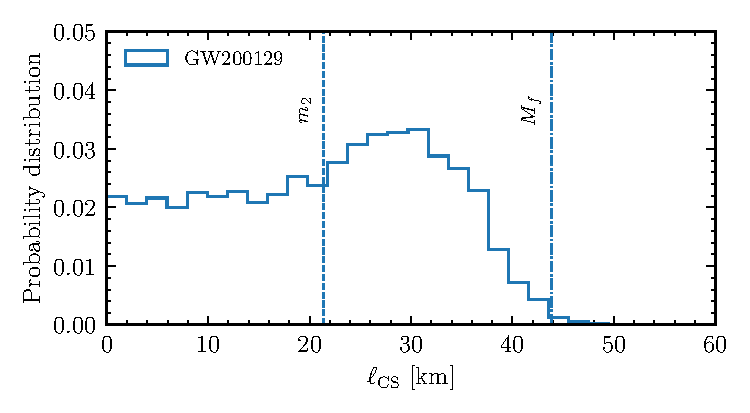
\includegraphics[width=\columnwidth]{figs/dcs_GW200129.pdf}
\caption{Posterior probability distribution on $\ell_{\rm CS}$ with GW200129.
The posterior shows that information was gained on this parameter relative to
the initial uniform prior distribution $\ell_{\rm CS} \in [0,\, 200]$~km.
%
The vertical lines represent two threshold for the validity of the theory as
an EFT.
%
The dotted line (labelled ``$m_2$'') at $\ell_{\rm CS} \approx 21.3$~km is
given by the median value of the secondary's mass $\varepsilon \, (G m_2 / c^2)$.
%
The dot-dashed line (labelled ``$M_{f}$'') at $\ell_{\rm CS} \approx 43.8$~km is
given by the median value of the remnant's mass $\varepsilon \, (G M_{f} / c^2)$.
%
For both, we used $\varepsilon = 0.5$.
%
If we take the latter as a length scale for the validity of dCS as an EFT, we
have place upper bound on $\ell_{\rm CS} \leqslant 43.8$~km, within the
approximation of our formalism.
}
\label{fig:dCS_bounds}
\end{figure}

\begin{figure}[t]
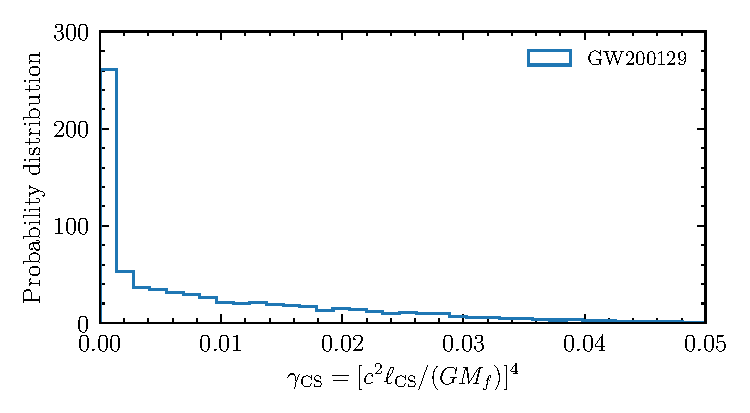
\includegraphics[width=\columnwidth]{figs/dcs_gamma_GW200129.pdf}
\caption{Posterior probability distribution on $\gamma_{\rm CS}$ with GW200129.
The posterior shows that the parameter $\gamma$ [see Eq.~\eqref{eq:def_gamma}]
in dynamical Chern-Simons has a peak at zero, indicating consistency with GR.
}
\label{fig:dCS_gamma_plot}
\end{figure}

%%%%%%%%%%%%%%%%%
\section{Discussion}
\label{sec:discussion}
%%%%%%%%%%%%%%%%%

\hs{I think an important message of the paper is that we give indication that
there are theories of gravity (such as dCS) which can by-pass observational
constraints from the inspiral phase alone, {\it yet} they do not, if we
analyze the ringdown. This is quite important because I've frequently heard
that the ``inspiral is what will constrain theories''. I think this might be
the most important message.}

%%%%%%%%%%%%%%%%%
\section*{Acknowledgements}
\label{sec:acknowledgements}
%
We thank Emanuele~Berti, Andrea~Maselli, Caio~F.~B.~Macedo, Deyan~Mihaylov, and
Serguei~Ossokine for discussions.
%
We thank the computational resources provided by the AEI, specifically the
{\sc Hypatia} cluster and Steffen Grunewald for assistance.
%
The authors would like to thank everyone at the frontline of the Covid-19
pandemic.
%%%%%%%%%%%%%%%%%

% \bibliographystyle{apsrev}
\bibliography{paper_alt_theor_bounds}

\end{document}
